\section{Structuur}
Deze sectie beschrijft de structuur van belangrijke en interessante onderdelen van het systeem. 
Deze beschrijvingen worden al dan niet ondersteund met een bijbehorend diagram indien dit van toepassing is.

\subsection{Leslokalen en vakken}
Volgend UML diagram beschrijft de structuur van de verscheidene klassen betreffende leslokalen en lessen die met elkaar gerelateerd zijn op het logisch niveau van het systeem.
Deze klassen bezitten data vanuit de databank die nodig zullen zijn om lessenroosters en examenroosters te plannen.

\begin{figure}[H]
	\centering
	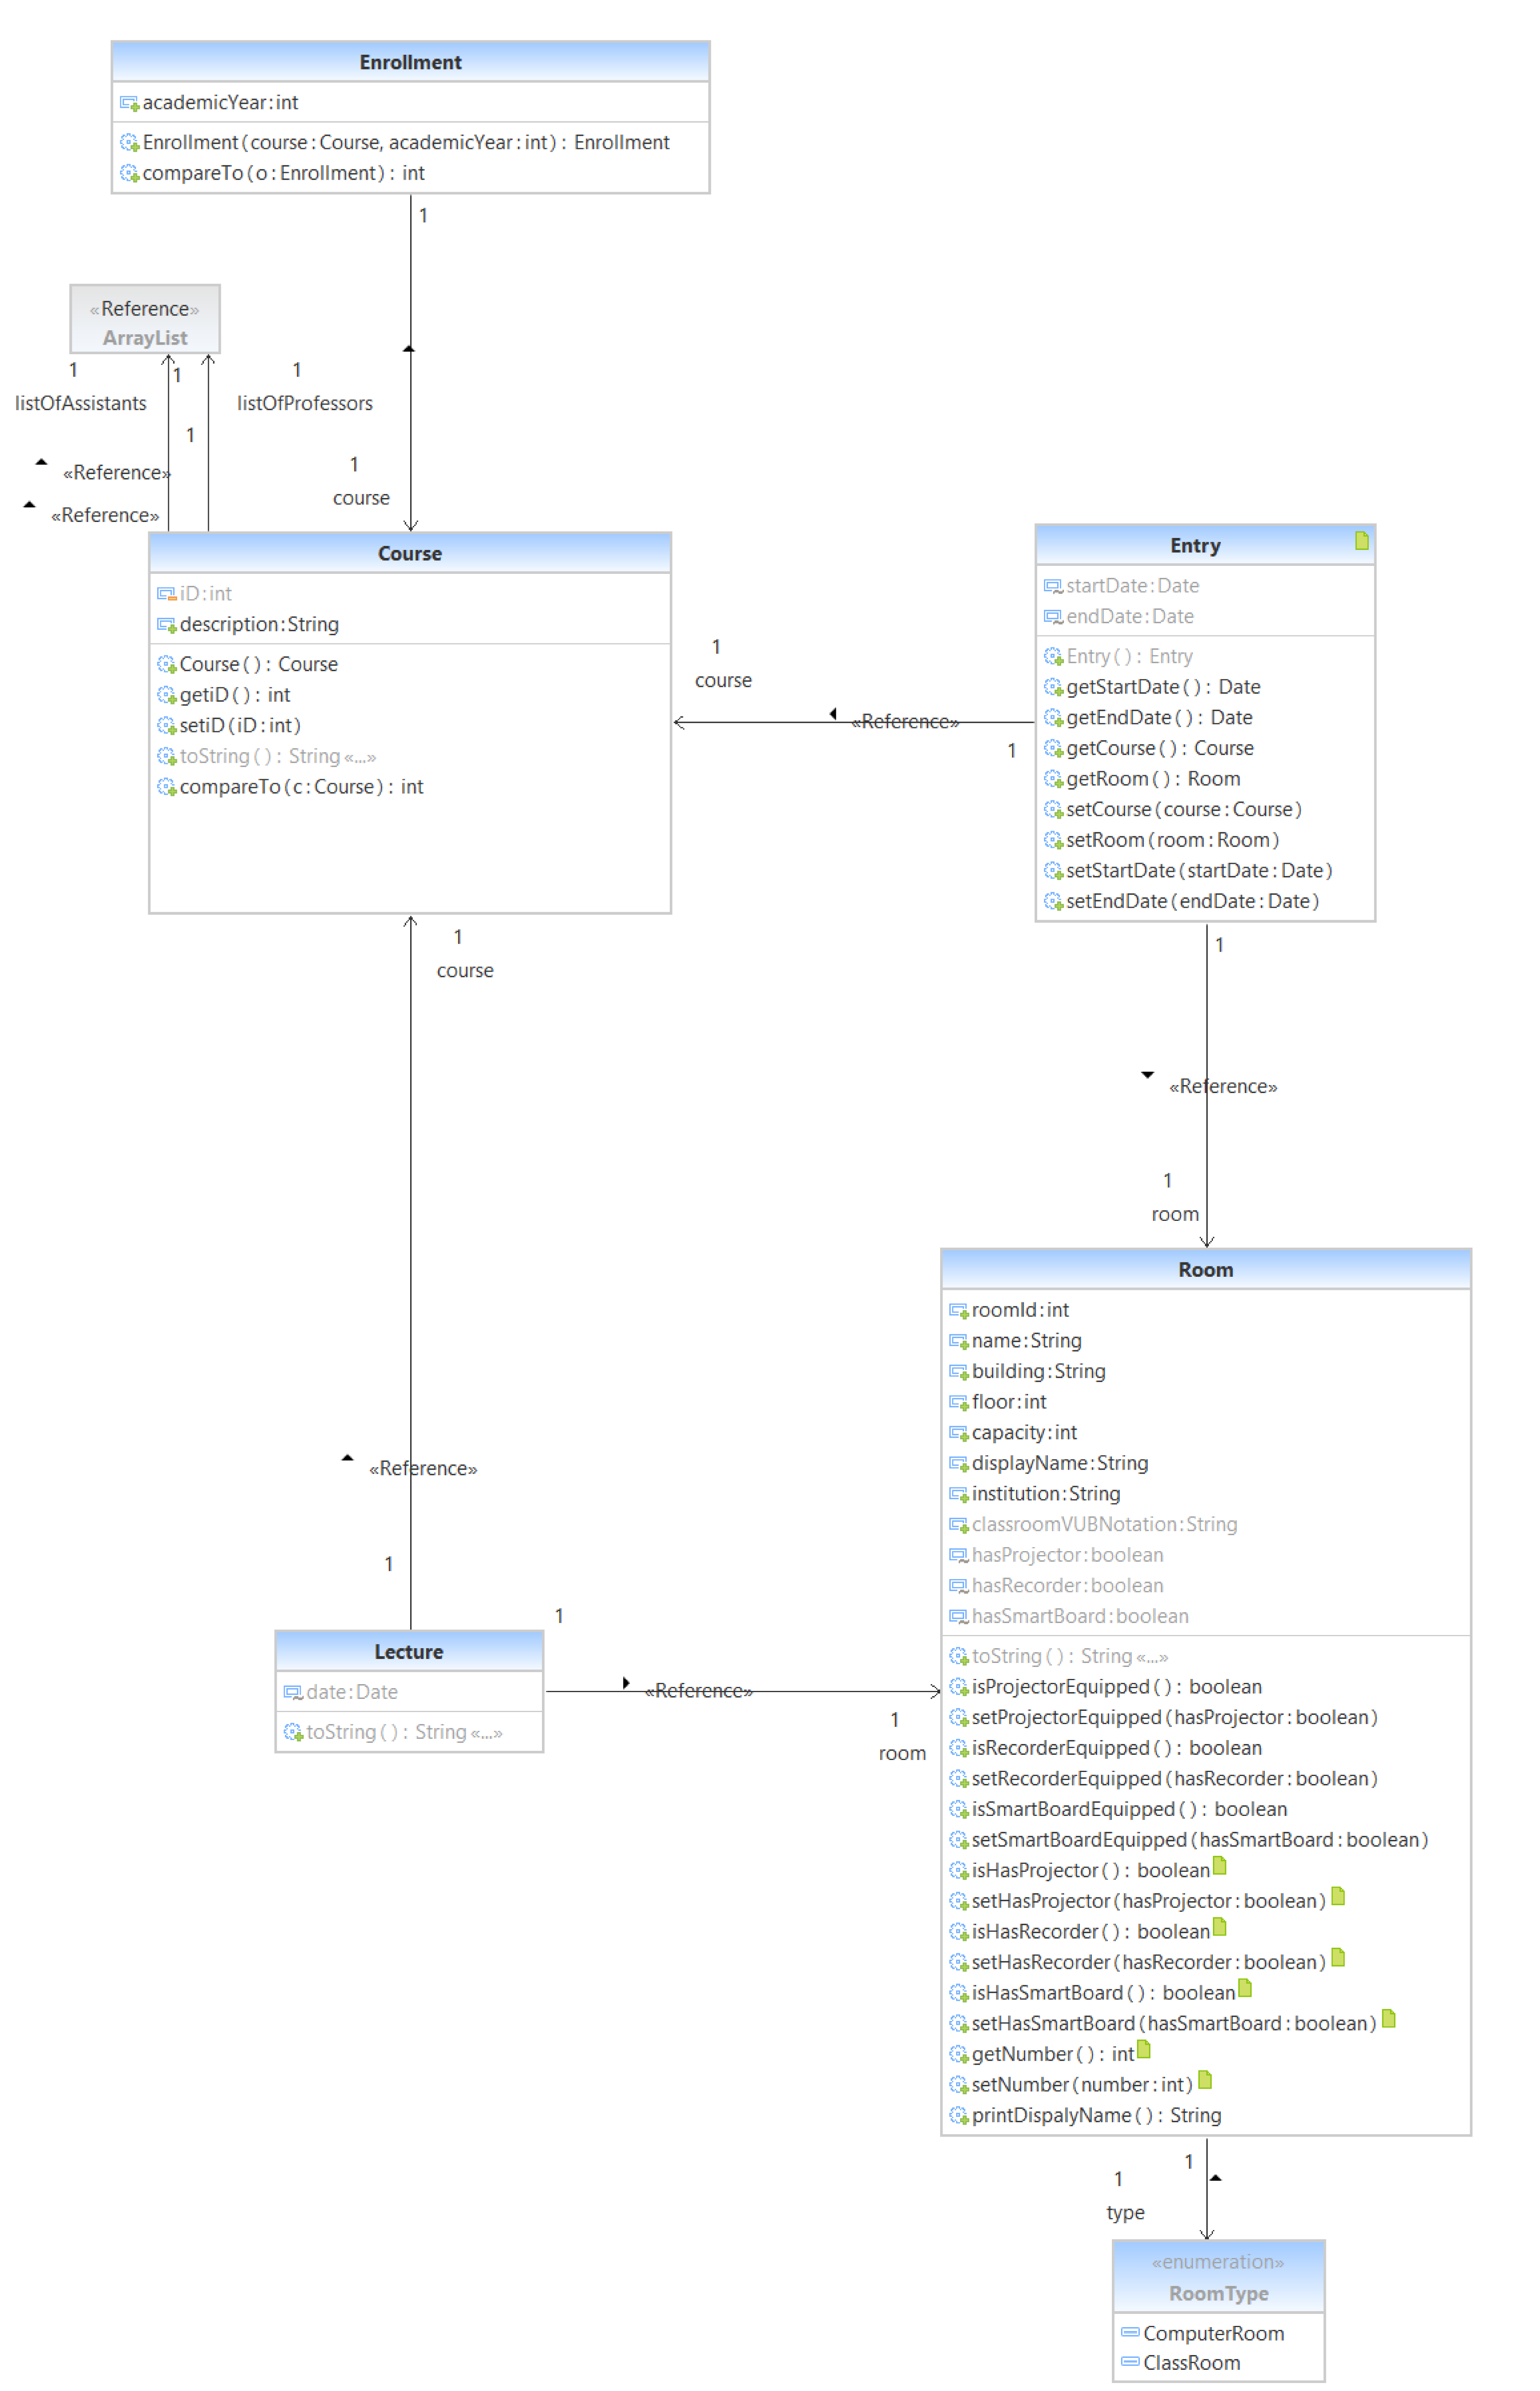
\includegraphics[scale=0.4]{img/roomsAndCourses}
	\caption{UML klassediagram voor leslokalen en vakken}
	\label{fig:roomsAndCourses}
\end{figure}

\subsection{Logging}
\label{subsec:logging}
Als logging framework werd gekozen voor SLF4J\cite{slf4j}.
Dit framework is echter een API die het maken van logs versimpelt voor de programmeur en vereist dus nog een geconfigureerde backbone.
Als backbone werd gekozen voor logback \cite{logback}.\\

In loggingsystemen kan men verschillende soorten logberichten produceren. 
Het systeem zorgt er dan voor dat deze berichten op de juiste plaats terecht komen.
De belangrijkste soorten berichten zijn: info, warning, error en debug.
In wat volgt wordt de configuratie van het loggingsysteem uitgeklaard.\\

Alle logberichten worden op de standaard output getoond.
Verder worden er specifieke logs opgeslagen naar bestanden.
Er zijn 2 folders voorzien voor logs: eentje voor debug logs en een folder met daarin een algemene log file.
Deze algemene log file bevat log berichten vanaf het niveau 'INFO', wat betekent dat het dus INFO, WARNING en ERROR logs bewaart.
Voor de debug logs wordt iedere dag een nieuwe file aangemaakt omdat het systeem een massa aan debug logs kan produceren op een dag.\\

Voor het in productie gaan van de applicatie is het sterk aangeraden de debug logs uit te schakelen om de lengte van de totale hoeveelheid logs drastisch te krimpen.

\subsection{Scheduler}
\subsubsection{Scheduling}
\label{subsec:scheduleclass}
Volgend UML klassediagram beschrijft de structuur van de klassen betreffende lessenroosters en het maken van zulke roosters.
Figuur \ref{fig:scheduling} beschrijft hoe het planningsprobleem in onze applicatie geformuleerd wordt.
Het framework OptaPlanner\cite{optaplanner} maakt gebruik van deze klassen door middel van annotaties om lessenroosters te maken.
Nu volgt een simpele beschrijving van de structuur.\\

Een \textit{Schedule} is een planning.
Zo een planning bestaat uit een sequentie van \textit{Entries}.
Een \textit{Entry} kan men vergelijken met een afspraak in een agenda.
In ons systeem wordt zo dus gevormd door een klaslokaal (Room), een vakonderdeel (CourseComponent) en een tijdstip (Date).
Een initialisatieklasse, \textit{SchedulerInitializer}, voorziet de beschikbare datums en tijdstippen.
Het verwezenlijken van een planning wordt opgelost door de klasse \textit{SchedulerSolver}.
Deze klasse zal gebruik maken van OptaPlanner om een \textit{ Schedule} te genereren.
Impliciet zal de \emph{SchedulerSolver} gebruik maken van de klassen \emph{SchedulerHelper}, \emph{EntryDifficultyComparator}, \emph{RoomStrengthComparator}, \emph{DateStrengthComparator} in een poging een zo goed mogelijk lessenrooster te bekomen.
De klasse \emph{MovableSelectionEntry} zorgt ervoor dat OptaPlanner weet welke entries verschoven mogen worden door de solver en welke niet.
Er is dus een notie van bevriezen van entries aanwezig in de schedule.
Meer uitleg over hoe OptaPlanner werkt en geconfigureerd is wordt beschreven in \ref{subsec:scheduling}.\\

De klasse \emph{SchedulerSolver} is een subtype van de klasse \emph{SchedulerScoreCalculator}.
Deze klasse is verantwoordelijk het berekenen van de score van een \emph{Schedule} in zijn huidige staat.
Via deze klasse kan men ook conflicten gaan detecteren.


Alle klassen in het klassenmodel, op de klasse \emph{HardSoftLongScore} na, diende zelf geschreven te worden en geannoteerd te worden zodat OptaPlanner deze klassen kon herkennen en gebruiken.
Bij het maken van deze klassen diende bepaalde interfaces van OptaPlanner ge\"{i}mplementeerd te worden, Solution\footnote{\url{https://docs.jboss.org/drools/release/6.0.1.Final/optaplanner-javadoc/org/optaplanner/core/impl/solution/Solution.html}} en ScoreDirector\footnote{\url{https://docs.jboss.org/drools/release/6.0.1.Final/optaplanner-javadoc/org/optaplanner/core/impl/score/director/ScoreDirector.html}} en werd de klasse HardSoftLongScore gebruikt.
In het klassediagram werden deze aangeduid met de annotatie \emph{$\langle\langle OPTAPLANNER\rangle\rangle$}.\\


\begin{landscape}
	\begin{figure}[H]
		\centering
		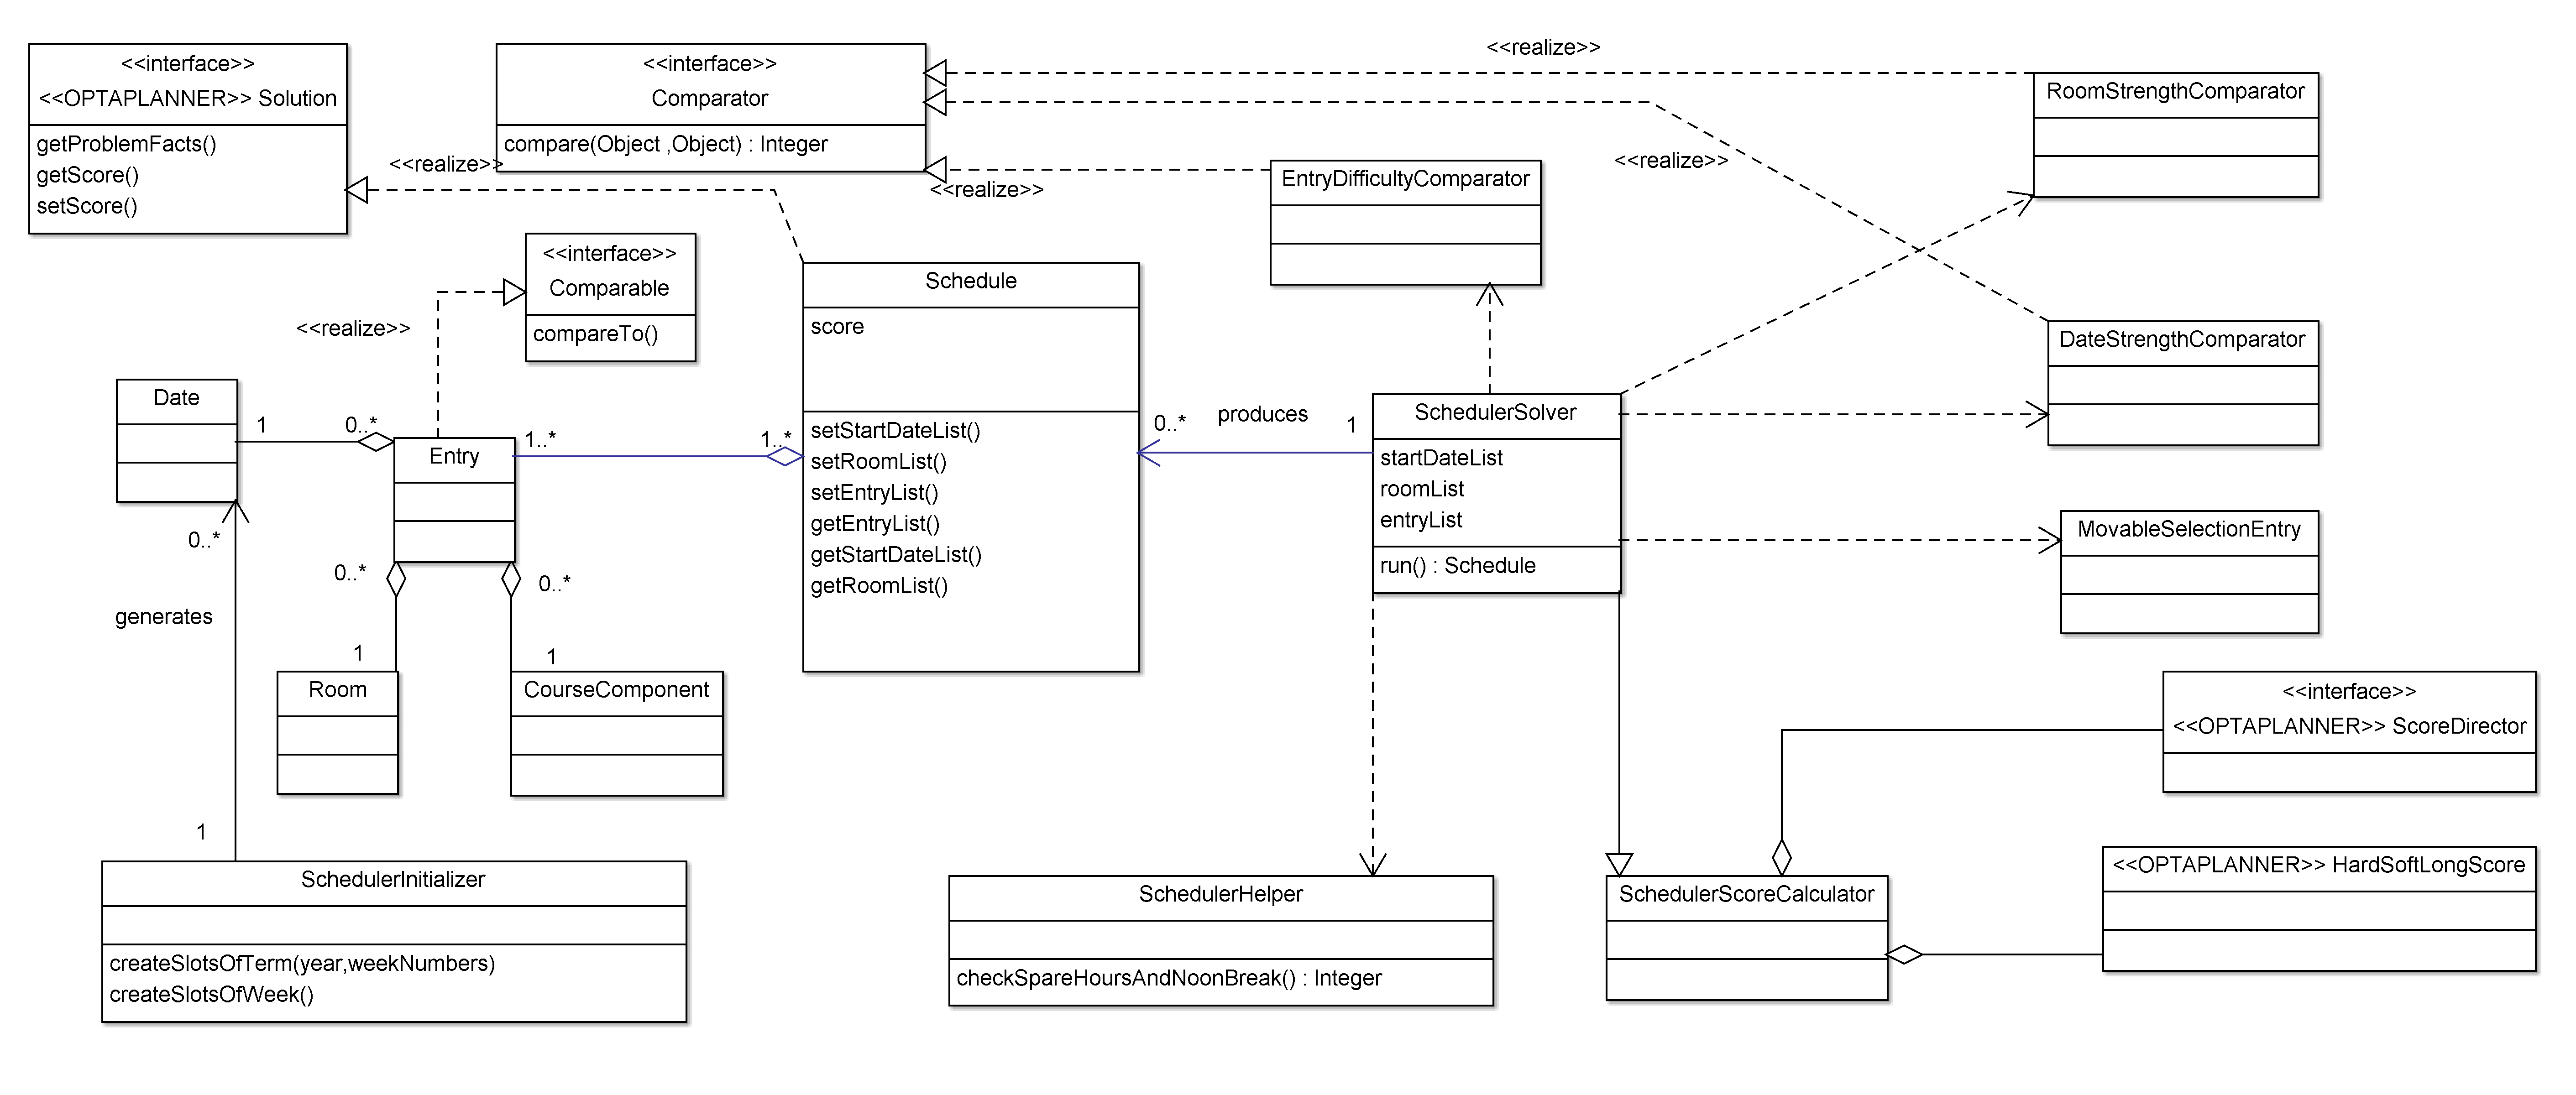
\includegraphics[scale=0.125]{img/scheduler}
		\caption{UML klassediagram voor scheduling}
		\label{fig:scheduling}
	\end{figure}
\end{landscape}

\subsubsection{Conflictdetectie in roosters}
\label{subsubsec:conflicts}
De interface \emph{ScoreDirector}\footnotemark[\value{footnote}] van OptaPlanner is verantwoordelijk om de score van de staat van een planningoplossing te berekenen.
Naast het berekenen van deze score, is de klasse ook in staat om te verklaren hoe hij aan die score komt. 
De \emph{ScoreDirector} voorziet een \emph{justificationList}, een lineaire structuur die informatie bevat over welke regels uit de Drools file afgevuurd zijn.
Aangezien deze regels declaratief zijn en er dus gebruik wordt gemaakt van pattern matching, staat er ook in de \emph{justificationList} welk patroon (de verzameling objecten die voldoet aan de match) er gevonden werd.\\

Dit stelt ons in staat deze informatie te parsen en te vertalen naar ons eigen design om conflicten in een schedule te melden aan de programmabeheerders en professoren die gebruik maken van CalZone.
Figuren \ref{fig:conflictdetection} en \ref{fig:constraintviolations} beschrijven de structuur van de objecten die dit tot stand brengen.\\

Een klasse \emph{ConstraintChecker} zal de \emph{justificationList} van de \emph{ScoreDirector} van OptaPlanner analyseren en een lijst van schendingen teruggeven.
Zo een schending wordt voorgesteld door de interface \emph{ConstraintViolation}.
Deze interface bezit een methode 'description'.
Deze methode geeft een string terug die het gehele conflict uitlegt.
De klasse \emph{ConstraintChecker} is dus het aanspreektpunt voor de front-end om conflicten in een bestaand rooster weer te geven aan gebruikers.\\

Voor iedere constraint is er een klasse voorzien die de interface \emph{ConstraintViolation} implementeert en dus een beschrijving ontwikkelt afhankelijk van wat voor constraint geschonden werd.\\

Het genereren van deze klasses voor de \emph{ConstraintChecker} wordt afgehandeld door een andere klasse: \emph{ConstraintViolationFactory}.

\begin{figure}[H]
	\centering
	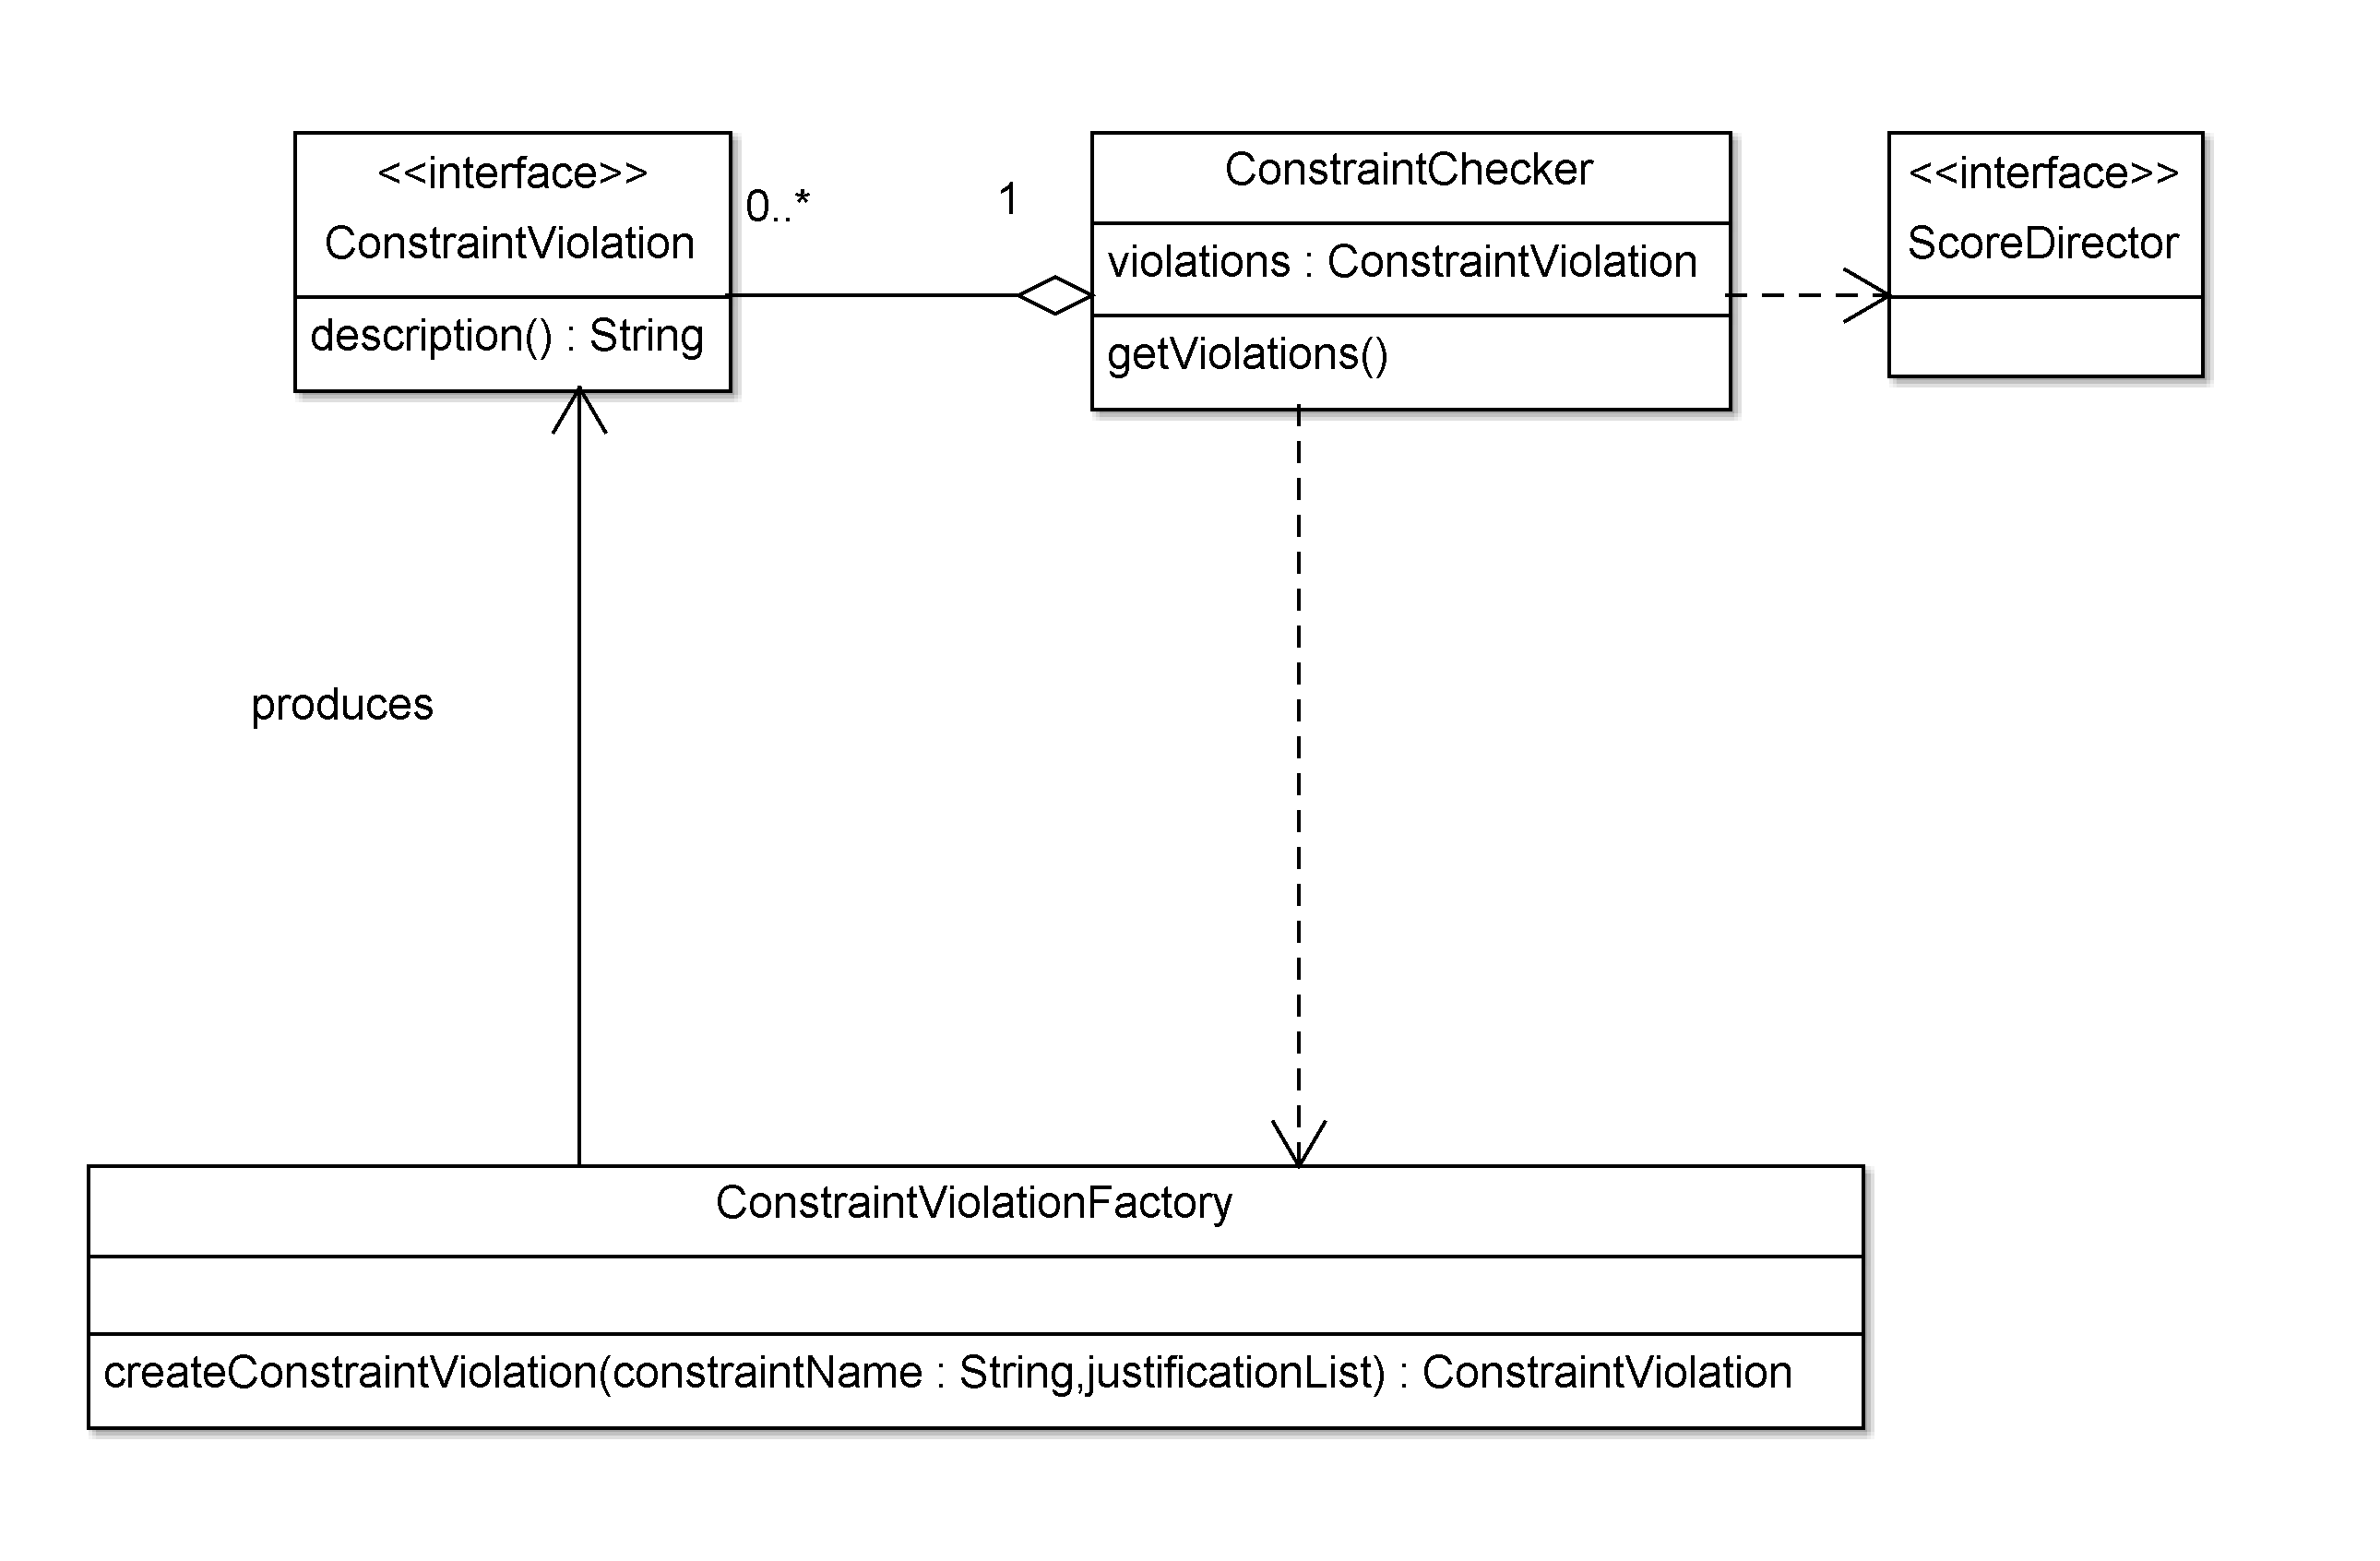
\includegraphics[scale=0.15]{img/conflictdetection}
	\caption{UML klassediagram voor conflictdetectie te realiseren}
	\label{fig:conflictdetection}
\end{figure}

 
\begin{figure}[H]
	\centering
	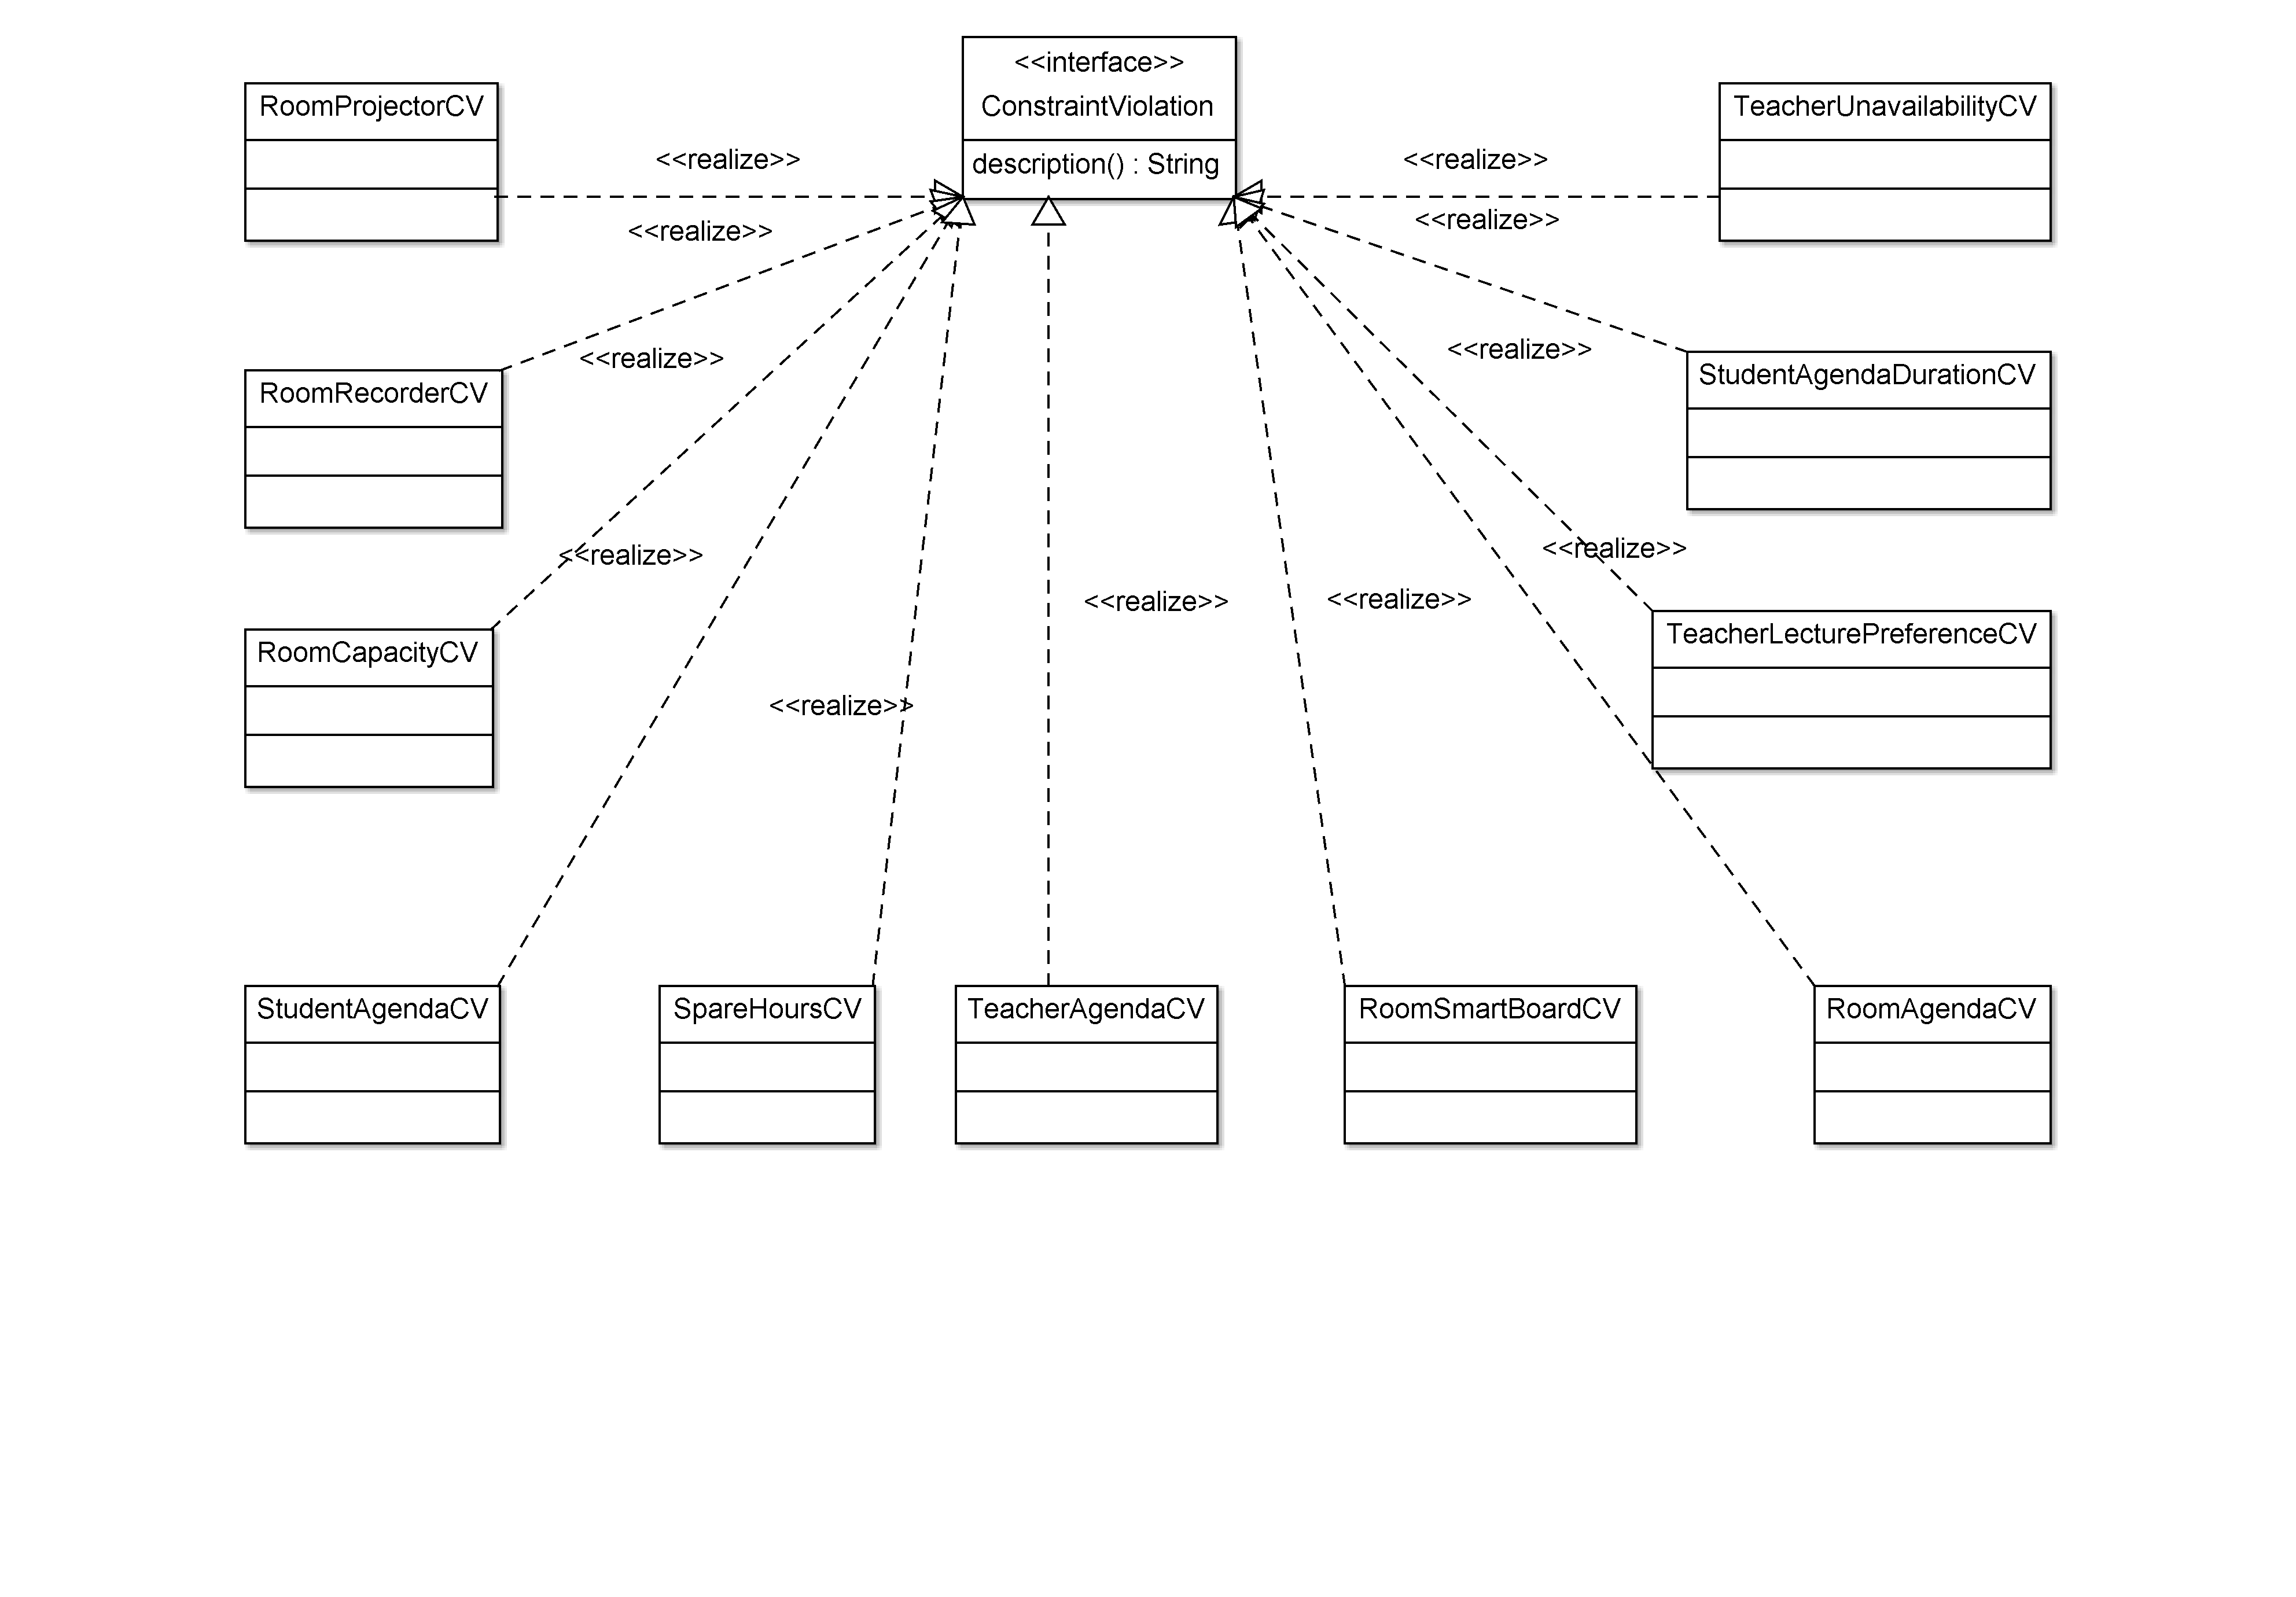
\includegraphics[scale=0.13]{img/constraintviolations}
	\caption{UML klassediagram van de verschillende ConstraintViolations}
	\label{fig:constraintviolations}
\end{figure}
